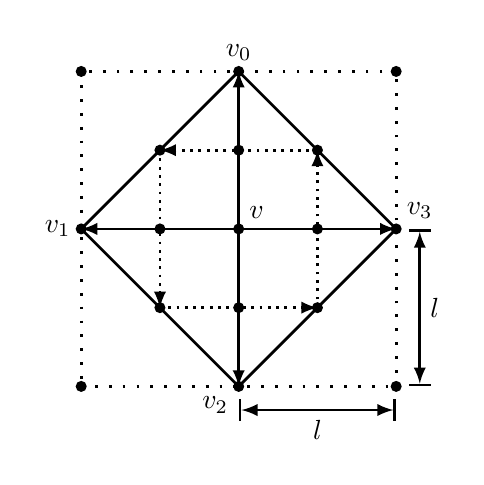
\begin{tikzpicture}[line width=1pt, >=latex]
	\coordinate (V) at (0,0);
	\coordinate (V0) at (0,2);
	\coordinate (V1) at (-2,0);
	\coordinate (V2) at (0,-2);
	\coordinate (V3) at (2,0);

	\fill (V) node[above right] {\(v\)} circle (2pt);
	\fill (V0) node[above] {\(v_0\)} circle (2pt);
	\fill (V1) node[left] {\(v_1\)} circle (2pt);
	\fill (V2) node[below left] {\(v_2\)} circle (2pt);
	\fill (V3) node[above right] {\(v_3\)} circle (2pt);

	\draw[->] (V) -- (V0);
	\draw[->] (V) -- (V1);
 	\draw[->] (V) -- (V2);
	\draw[->] (V) -- (V3);

	\draw (V0) -- (V1);
	\draw (V1) -- (V2);
	\draw (V2) -- (V3);
	\draw (V3) -- (V0);

	\coordinate (W0) at (-2,2);
	\coordinate (W1) at (-2,-2);
	\coordinate (W2) at (2,-2);
	\coordinate (W3) at (2,2);

	\fill (W0) circle (2pt);
	\fill (W1) circle (2pt);
	\fill (W2) circle (2pt);
	\fill (W3) circle (2pt);

	\draw[style=loosely dotted] (W0) -- (W1);
	\draw[style=loosely dotted] (W1) -- (W2);
	\draw[style=loosely dotted] (W2) -- (W3);
	\draw[style=loosely dotted] (W3) -- (W0);

	\coordinate (C01) at (-1,1);
	\coordinate (C12) at (-1,-1);
	\coordinate (C23) at (1,-1);
	\coordinate (C30) at (1,1);

	\fill (C01) circle (2pt);
	\fill (C12) circle (2pt);
	\fill (C23) circle (2pt);
	\fill (C30) circle (2pt);

	\draw[->, style=dotted] (C01) -- (C12);
	\draw[->, style=dotted] (C12) -- (C23);
	\draw[->, style=dotted] (C23) -- (C30);
	\draw[->, style=dotted] (C30) -- (C01);

	\coordinate (C0) at (0,1);
	\coordinate (C1) at (-1,0);
	\coordinate (C2) at (0,-1);
	\coordinate (C3) at (1,0);

	\fill (C0) circle (2pt);
	\fill (C1) circle (2pt);
	\fill (C2) circle (2pt);
	\fill (C3) circle (2pt);


	\draw[|<->|] (0,-2.3) -- node[below] {\(l\)} (2,-2.3);
	\draw[|<->|] (2.3,0) -- node[right] {\(l\)} (2.3,-2);
	
	\useasboundingbox ([shift={(1mm,1mm)}]current bounding box.north east) rectangle ([shift={(-1mm,-1mm)}]current bounding box.south west);
\end{tikzpicture}